\documentclass[12pt]{article}

\usepackage[utf8]{inputenc}
\usepackage[T1]{fontenc}
\usepackage{mathptmx}
\usepackage[margin=1in]{geometry}
\usepackage{graphicx}
\usepackage{caption}
\usepackage[hidelinks]{hyperref}

\captionsetup{font=small, labelfont=bf}
\setlength{\parindent}{0pt}
\setlength{\parskip}{6pt}
\newcommand{\deltaauc}{$\Delta$AUC}

\title{}
\date{}

\begin{document}

\begin{center}
{\large\bfseries Figures}\\[2pt]
{\small Reported biomarker--cognition associations do not translate into predictive utility: a pre-registered analysis of NHANES 2011--2014}\\[2pt]
{\small Shreyan Kancharla, Neil Patel}
\end{center}

\bigskip

\begin{figure}[htbp]
\centering
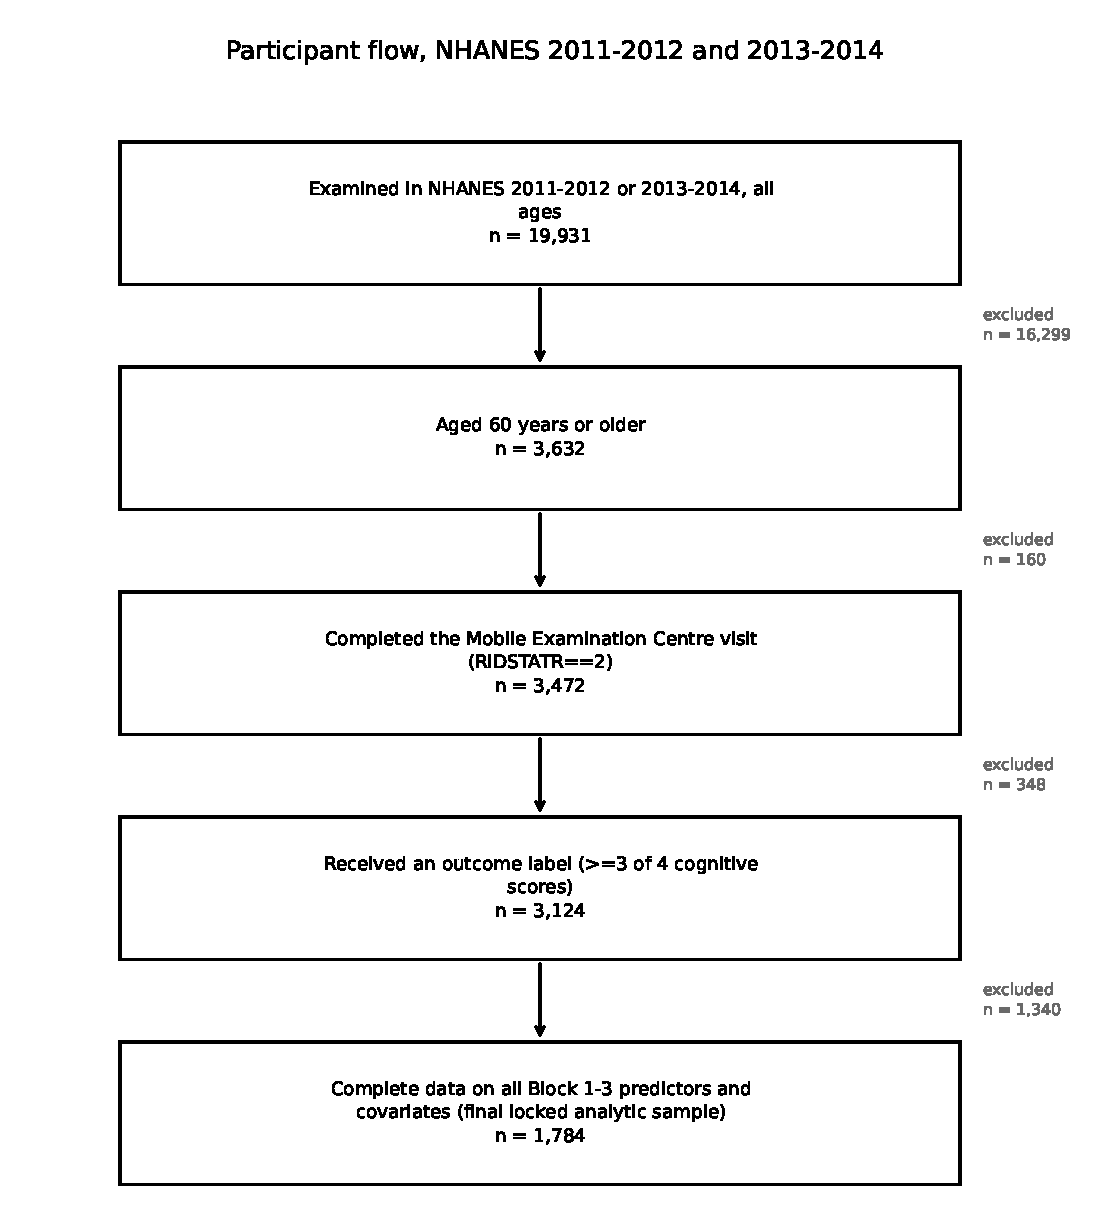
\includegraphics[width=0.85\textwidth]{figures/fig6_participant_flow.pdf}
\caption{Participant flow from NHANES 2011--2012 and 2013--2014 examined participants to the final locked analytic sample. Reasons for exclusion are given at each stage; the final step's exclusions (missing predictor data) are not mutually exclusive across blocks.}
\label{fig:flow}
\end{figure}

\clearpage
\begin{figure}[htbp]
\centering

\includegraphics[width=0.95\textwidth]{figures/fig1_delta_auc_forest.pdf}
\caption{Forest plot of \deltaauc\ contrasts with bootstrap 95\% confidence intervals: the four primary nested contrasts (M1$-$M0, M2$-$M0, M3$-$M0, M3$-$M0+) and the six pre-specified sensitivity analyses for M3$-$M0. Red markers indicate intervals excluding zero. The shaded band marks the pre-specified 0.02 meaningful-difference threshold.}
\label{fig:forest}
\end{figure}

\clearpage
\begin{figure}[htbp]
\centering

\includegraphics[width=0.7\textwidth]{figures/fig2_calibration.pdf}
\caption{Calibration, out-of-fold, by decile of predicted probability, for M0 (demographics), M3 (all biomarkers) and M0+ (clinical baseline). Calibration slope for each model is given in the legend; the dashed line is perfect calibration.}
\label{fig:calibration}
\end{figure}

\clearpage
\begin{figure}[htbp]
\centering
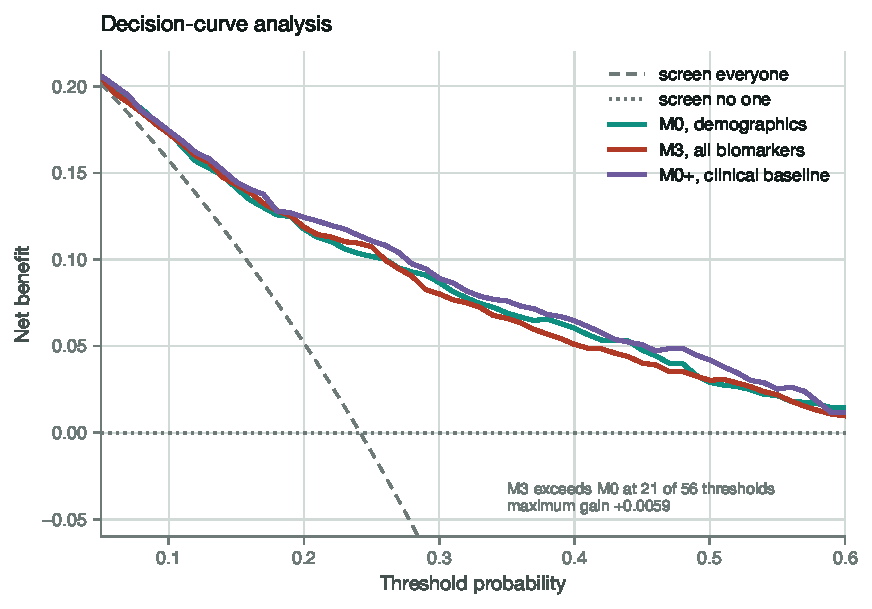
\includegraphics[width=0.85\textwidth]{figures/fig3_decision_curve.pdf}
\caption{Decision-curve analysis: net benefit against threshold probability for M0, M3 and M0+, against the treat-all and treat-none reference strategies.}
\label{fig:dca}
\end{figure}

\clearpage
\begin{figure}[htbp]
\centering

\includegraphics[width=0.9\textwidth]{figures/fig4_shap_rank_stability.pdf}
\caption{SHAP feature-importance rank stability across 200 bootstrap resamples of the gradient-boosted M3 model. Points are median rank, bars are the 95\% interval; the right-hand column gives the percentage of resamples in which each feature appeared in the top 5. Demographic predictors (purple) are essentially deterministic in rank; biomarkers (teal) are not.}
\label{fig:shap}
\end{figure}

\clearpage
\begin{figure}[htbp]
\centering
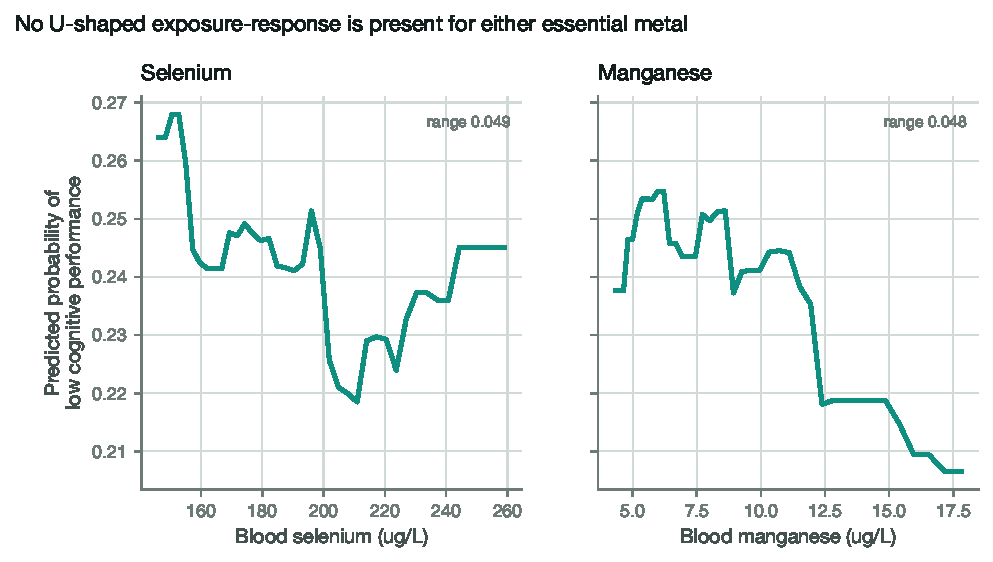
\includegraphics[width=0.9\textwidth]{figures/fig5_partial_dependence.pdf}
\caption{Partial dependence of predicted probability of low cognitive performance on blood selenium and blood manganese concentration (gradient-boosted M3 model), the two exposures for which a non-monotonic (U-shaped) exposure-response was anticipated in advance. Neither shows one; the predicted probability varies by approximately 0.05 across each exposure's observed range.}
\label{fig:pdp}
\end{figure}

\end{document}
